\subsection{Target Density}\label{sec:analysis.target_density}

We need to know the target density to calculate the differential cross-section. The procedure for determining the density of $\ell$H$_2$ target in \abbr{CLAS} has already been established\cite{clas.target.density}. In the \desg{g12} experiment, the target temperature and pressure was measured periodically during each run. Each run contained at least 3 measurements of the pressure and temperature. The formula for calculating the target density is:
\begin{align}
\rho = a_1 T^2 + a_2 P + a_3,
\label{eq:target_density}
\end{align}
where $T$ and $P$ represent the temperature and pressure respectively and $a_1$, $a_2$, $a_3$ are constants given in Tab.~\ref{tab:targetdensity} taken from Ref.~\cite{clas.target.density}. Fig.~\ref{fig:target_density} shows the average target density, $\bar \rho$, for each run along with the $\sqrt{\sigma^2}$.
\begin{table}[h!]
\begin{minipage}{\textwidth}
\begin{center}
\begin{singlespacing}

\caption[Target Density Constants]{\label{tab:targetdensity}Constants used in target density measurements \vspace{0.75mm}}

\begin{tabular}{c|c}

%\hline \hline
%
%operation & \multicolumn{3}{c}{Generation} \\
%charge & I & II & III \\

\hline
Parameter & Value \\
\hline

$a_{1}$ & $-2.89 \cdot 10^{-5} \frac{g}{cm^3K^2}$  \\
$a_{2}$ & $1.0 \cdot 10^{-7} \frac{g}{cm^3mbar}$  \\
$a_{3}$ & $8.249 \cdot 10^{-2} \frac{g}{cm^3}$  \\
\hline \hline
\end{tabular}

\end{singlespacing}
\end{center}
\end{minipage}
\end{table}
\vspace{20pt}
The average density, for each run, was calculated as;
\begin{align}
\bar \rho_{run} = \frac{1}{N}\sum_i^N \rho_i,
\end{align}
while the variance $\sigma^2$ is calculated, for each run, as;
\begin{align}
\sigma^2 = \frac{1}{N - 1}\sum_i^N (\rho_i - \bar \rho)^2.
\end{align}
Once the target density was calculated for each run, the average target density for all \desg{g12} runs was calculated using;
\begin{align}
\bar \rho_{tot} = \frac{1}{N_{run}}\sum_i^{N_{run}} \bar \rho_{run} = 0.0711398 \pm 1.74 \cdot10^{-5},
\end{align}
while the variance $\sigma^2$ is calculated, for all \desg{g12} run, as;
\begin{align}
\sigma_{tot}^2 = \frac{1}{N_{run} -1}\sum_i^{N_{run}} (\bar \rho_{run} - \bar \rho_{tot})^2 = 0.00024.
\end{align}
Since the uncertainty, σ, in the target density is lower than the uncertainty of the physical dimensions in the target materials, the target density uncertainty will not be a factor in the total systematic uncertainties.

\begin{figure}[htpb]\begin{center}
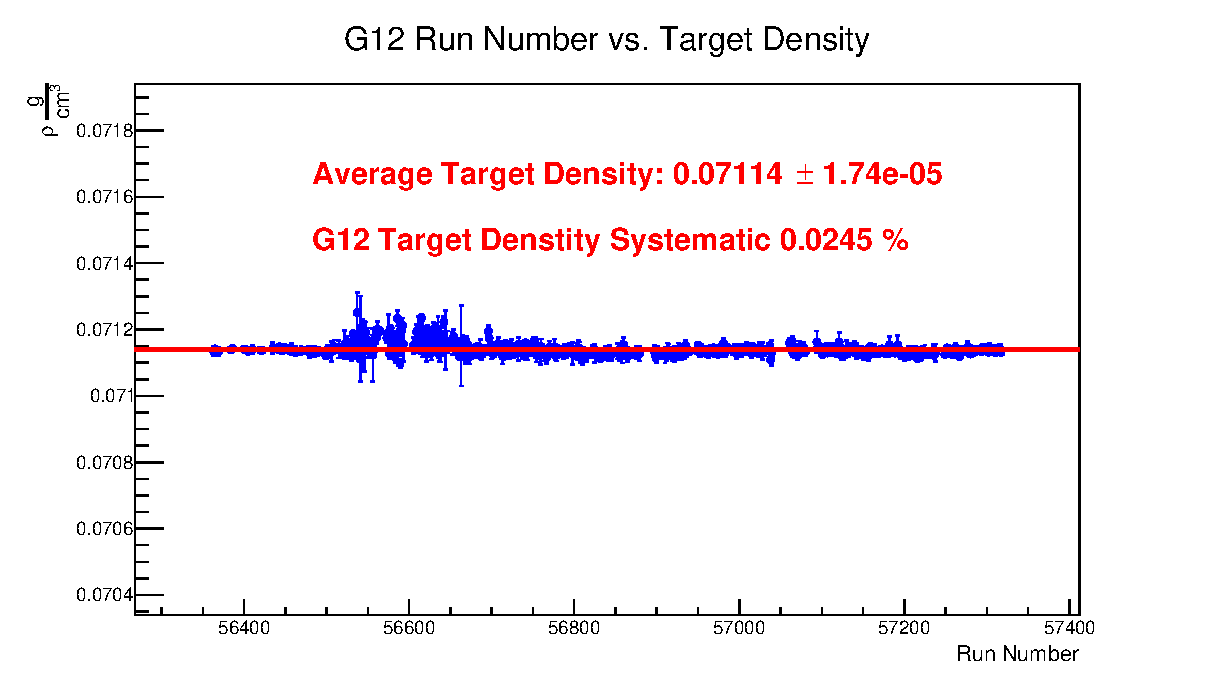
\includegraphics[width=0.9\textwidth]{figures/calib/targ/G12_Target_Density.eps}
\caption[Target density for \desg{g12}]{\label{fig:target_density}Target density for \desg{g12}. Image source:~\cite{clas.thesis.kunkel}}
\end{center}\end{figure}
\FloatBarrier

The systematic uncertainties relating to the target in fact also must account the effect such as the contraction, length, etc. Prior experiments such as eg2 have already established that the overall related effect is about $1\%$~\cite{eg2target}, which is also what g12 would use for the overall systematic uncertainty related to target. We do 	not see that there is any statistical significant data from the target cell walls, 	and do not subtract a background from the target cell walls. Standard g12 analysis 	should choose events from within the target, taking into account the contraction. 	If a particular 	analysis  chose to cut outside of the target, they would have do the 	systematics study accordingly. 